%type de document
\documentclass[a4paper,12pt]{article}

% regles typographiques françaises
%\usepackage[latin1]{inputenc}
\usepackage[utf8]{inputenc}
\usepackage[francais]{babel}
\usepackage[T1]{fontenc}


% mise en page
\usepackage[margin=2.5cm]{geometry}
\usepackage{fancyhdr}
\usepackage{graphicx}
\usepackage{array}
%\usepackage{lastpage}
%\usepackage{placeins}
%\usepackage{longtable}
%\usepackage{caption}
\usepackage{float}
\usepackage{wrapfig}
\usepackage{dirtree}

\usepackage[smaller, footnote, printonlyused]{acronym} % table d'acronymes, option [footnote] pour avoir les définitions en bas de page [printonlyused

\usepackage{hyperref}
\hypersetup{colorlinks=true, linkcolor=blue}
\hypersetup{pdfauthor=Sebastien Chassot}
\hypersetup{pdfstartpage=1}
\hypersetup{pdfpagemode=None} %FullScreen, None
\hypersetup{pdfpagelayout=SinglePage} %SinglePage, OneColumn, TwoColumnLeft, TwoColumnRight
\hypersetup{pdfstartview=FitH} %Fit, FitH, FitV, FitB, FitBH, FitBV
\pdfcompresslevel=9
%\hypersetup{
%  bookmarks=true                % show bookmarks bar?
%, bookmarksopen=true
%, unicode=false                 % non-Latin characters in Acrobat bookmarks
%, pdftoolbar=true               % show Acrobat toolbar?
%, pdfmenubar=true               % show Acrobat menu?
%, pdffitwindow=false            % window fit to page when opened
%, pdfpagemode=UseOutlines       % FullScreen, UseThumbs(show thumbnails)
%                                % UseOutlines(show bookmarks), None
%, pdfpagelayout=SinglePage      % SinglePage, OneColumn, TwoColumnLeft, TwoColumnRight
%, pdfstartpage=1
%, pdfstartview={FitV}           % Fit, FitH, FitV, FitB, FitBH, FitBV
%, pdfsubject={}
%, pdftitle={Rapport}    		% title
%, pdfauthor={J. Mendes, S. Chassot, D. Wittwer}       	% author
%, pdfcreator={LaTeX}            % creator of the document
%, pdfkeywords={HEPIA} {Rapport} {analyse} {programmation} {terminal} {c}  % list of keywords
%, pdfnewwindow=true             % links in new window
%, colorlinks=false              % false: boxed links; true: colored links
%, linkcolor=red                 % color of internal links
%, citecolor=black               % color of links to bibliography
%, filecolor=magenta             % color of file links
%  urlcolor=blue                 % color of external links
%}

% Espacement interligne
\usepackage{setspace}
\onehalfspacing

% Couleur
\usepackage{colortbl}
\definecolor{bleuClair}{rgb}{0.31,0.51,0.74}

% ligne vide
\newcommand{\emptyLine}[1][1]{\par\leavevmode\par}

% lstlisting configuration
\usepackage{fancyvrb}
\usepackage{xcolor}
\usepackage{listings}

% D�finition des couleurs
\definecolor{lightgreen}{rgb}{0.2,.98,0.2}
\definecolor{darkgreen}{rgb}{0,0.4,0}
\definecolor{lightgray}{gray}{0.98}
\definecolor{darkred}{rgb}{0.545,0.000,0.000}
\definecolor{bleuClair}{rgb}{0.31,0.51,0.74}
\definecolor{grisTableau}{rgb}{0.9529,0.9529,0.9529}
\lstset {	
  language=C
, frame=single
, keepspaces=true
, columns=fullflexible
, captionpos=b
, stepnumber=10
, morekeywords={var,get,set}
, basicstyle=\ttfamily\scriptsize
, keywordstyle=\color{blue}
, commentstyle=\color{darkgreen}
, stringstyle=\color{darkred}
, backgroundcolor=\color{white}
, numbers=left
, numberstyle=\scriptsize
, numbersep=5pt
, breaklines=true
, tabsize=3
, showstringspaces=false
, emph={double,bool,int,unsigned,char,true,false,void,get,set}
, emphstyle=\color{blue}
, emph={Assert,Test}
, emphstyle=\color{red}
, emph={[2]\#using,\#define,\#ifdef,\#endif}
, emphstyle={[2]\color{blue}}
, rulesepcolor=\color{gray}
, lineskip={-1.5pt} % single line spacing
, escapeinside={/*(*@}{@*)*/}
, rangeprefix=\{\  % curly left brace plus space
, rangesuffix=\ \} % space plus curly right brace
}
\lstset{prebreak=\raisebox{0ex}[0ex][0ex]
        {\ensuremath{\hookleftarrow}}}
%\lstset{postbreak=\raisebox{0ex}[0ex][0ex]
%        {\ensuremath{\hookrightarrow\space}}}
\lstset{breaklines=true, breakatwhitespace=true}

% replace sequence of char by another sequence of char
% see http://stackoverflow.com/questions/1116266/listings-in-latex-with-utf-8-or-at-least-german-umlauts
\lstset{literate=%
{ä}{{\"a}}1
{â}{{\^a}}1
{� }{{\`a}}1
{ë}{{\"e}}1
{ê}{{\^e}}1
{é}{{\'e}}1
{è}{{\`e}}1
{ï}{{\"i}}1
{î}{{\^i}}1
{ö}{{\"o}}1
{ô}{{\^o}}1
{ü}{{\"u}}1
{û}{{\^u}}1
{ç}{{\c c}}1
{°}{{\textsuperscript{o}}}1
% suppress BOM (Byte Order Mark) characters at the beginning of Visual Studio source
% see http://tex.stackexchange.com/questions/5935/how-to-suppress-bom-effect-in-the-output
{�}{}0
{�}{}0
{�}{}0
}

%%%%%%%%%%%%%%%%%%%%%%%%%%%%%%%%%%%%%%%%%%%%%%%%%%%%%%%%%%%%%%%%%
%		DEBUT DU DOCUMENT
%%%%%%%%%%%%%%%%%%%%%%%%%%%%%%%%%%%%%%%%%%%%%%%%%%%%%%%%%%%%%%%%%

\begin{document}

%%%%%%%%%%%%%%%%%%%%%%%%%%%%%%%%%%%%%%%%%%%%%%%%%%%%%%%%%%%%%%%%%%%
%		ENTETE ET PIED DE PAGE
%%%%%%%%%%%%%%%%%%%%%%%%%%%%%%%%%%%%%%%%%%%%%%%%%%%%%%%%%%%%%%%%%
\pagestyle{fancy}
% entête
\lhead{}
\chead{}
\rhead{}
% pied de page
\lfoot{}
\cfoot{Page \thepage\ sur \pageref{LastPage} }
\rfoot{}
\renewcommand{\headrulewidth}{0.1pt}
\renewcommand{\footrulewidth}{0.1pt}
\fancyhead[R]{\textsl{ prog system - TP Minix File system }}
%\fancyfoot[C]{\scriptsize\emph{\class}}

\fancyfoot[L]{\scriptsize\emph{\docschool{}}}


%%%%%%%%%%%%%%%%%%%%%%%%%%%%%%%%%%%%%%%%%%%%%%%%%%%%%%%%%%%%%%%%%%%

\author{Sebastien Chassot}
\newcommand{\docschool}{hepia - ITI}
\title{Rapport}

% page de titre
\begin{center}
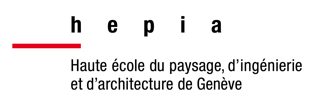
\includegraphics[scale=2]{imgs/hepia}
\end{center}

\vspace{3cm}

\begin{center}
\begin{huge}
\textbf{Rapport}
\end{huge}
\end{center}

\begin{center}
\begin{large}
Minix File system
\end{large}
\end{center}

% Trait de separation
\newcommand{\lineunder}{\color{bleuClair}\hrulefill\\\color{black}}
\lineunder

\begin{center}
\begin{large}
ITI 2\up{ème} soir \\
2014 / 2015
\end{large}
\end{center}

\vspace{3cm}
\centerline{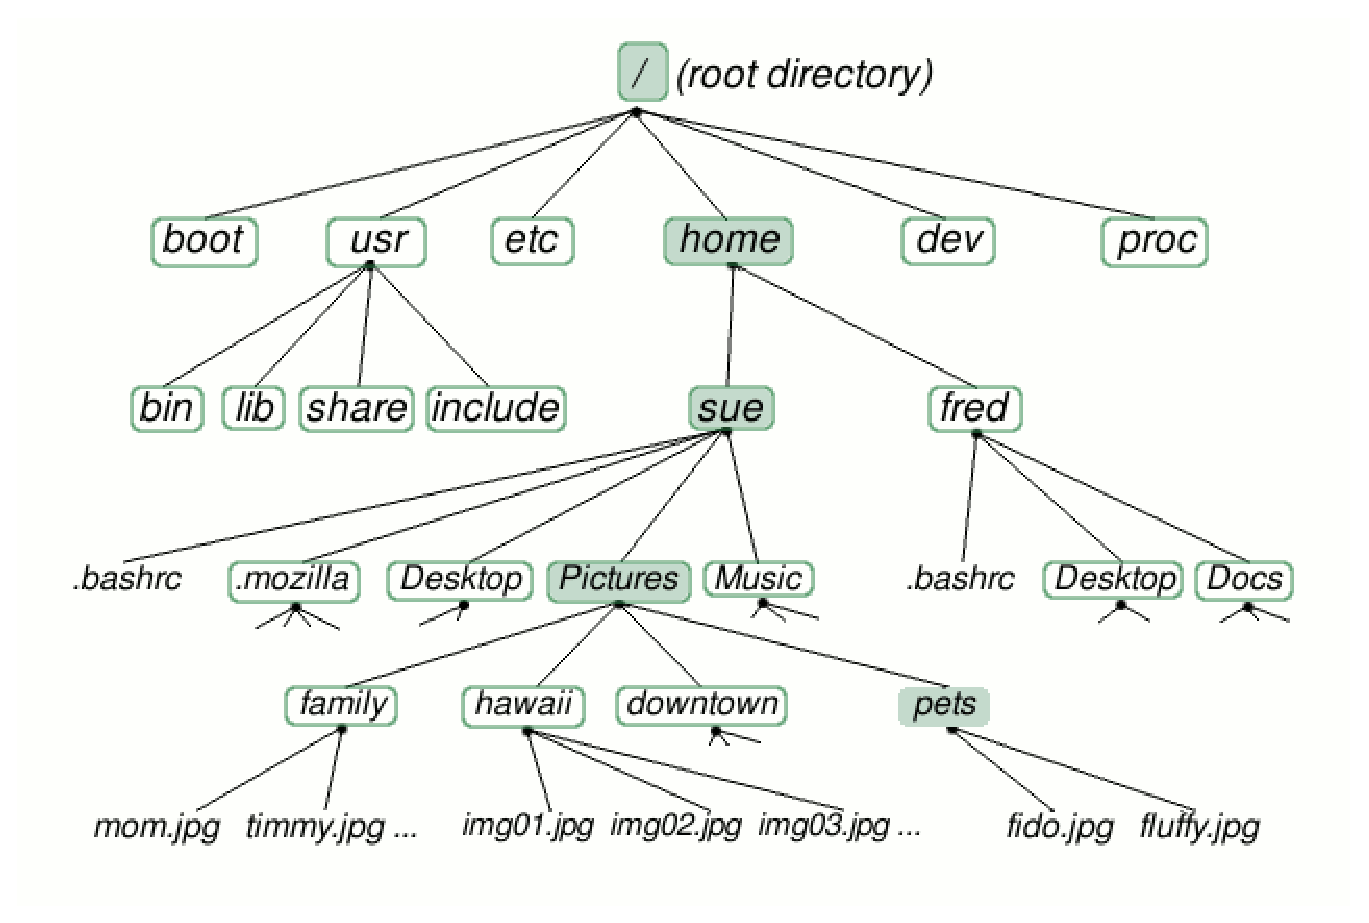
\includegraphics[scale=0.52]{imgs/illustration_FS}}
\vspace{2cm}

\begin{center}
%\begin{large}
\textbf{Sebastien Chassot} \\ Juin 2015
%\end{large}
\end{center}

\thispagestyle{empty} % enleve les entetes et pide de page de la page de titre

% table des matières
\newpage % nouvelle page
\tableofcontents % table des matières
\listoffigures
\listoftables
\newpage % nouvelle page

%\chapter*{Mini Bash}


\section{Introduction}

Le but de ce travail est d'implémenter un système MinixFS V1 en python en proposant une API standard et de modifier un fichier \emph{formaté} en minixfs via cet interface.\\

Dans un deuxième temps, les modifications seront faites à  travers le réseau. Un server (écrit en C) modifiera le fichier par block reçu via des sockets AF\_INET. On réutilisera le travail fait en python et son API mais les block seront transmis au server selon un protocole relativement simple.
 
\begin{figure}[H]
\begin{center}
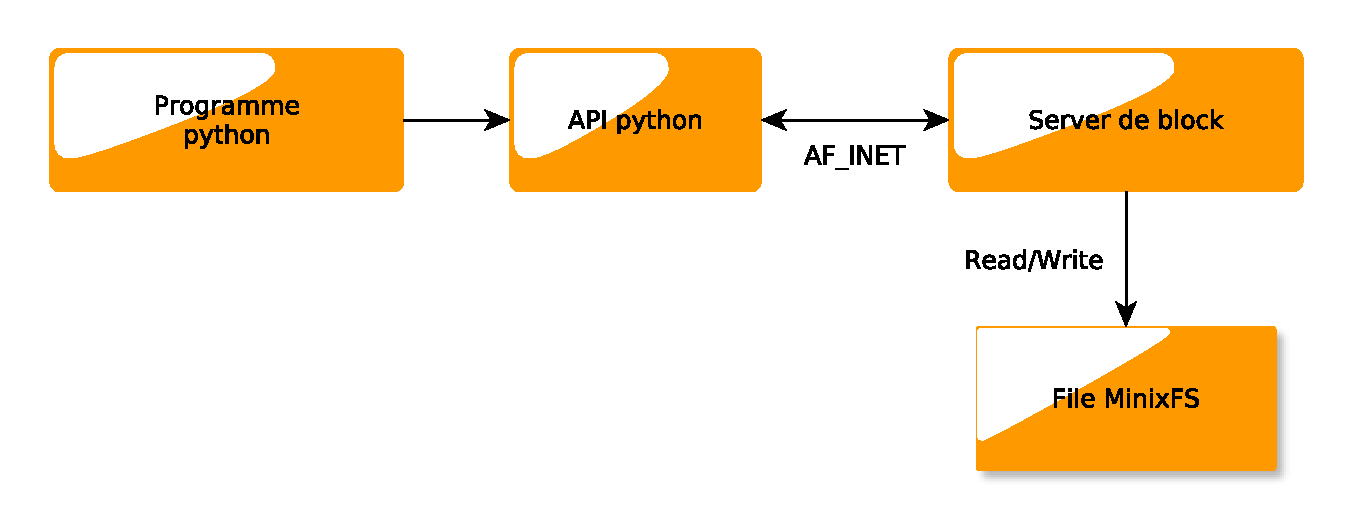
\includegraphics[scale=.6]{imgs/schema_client_server}
\caption{Principe de fonctionnement}
\label{fig:Architecture client server}
\end{center}
\end{figure}


Un seul client est traité à la fois ce qui évite les problèmes d'accès concurrent - traité dans d'autres cours. Le principe est simple. le client fait une requête, le server y répond.\\



\section{Implémentation python}

\subsection{description de l'API}


\begin{description}
\item[ialloc()] \hfill \\
	alloue un inode
\end{description}
\begin{itemize}
\item ialloc()
\end{itemize}



\subsection{ialloc()}

\begin{lstlisting}[language=C, caption=pseudo code ialloc()()]
ialloc(){

	recherche premier libre dans inode_map
	
	si not trouve:
		raise error plus aucun inode de libre
	
	inode trouve = occupe
	del ancien inode
	new inode
	
	return numero inode
}
\end{lstlisting}

\subsection{ifree()}

\begin{lstlisting}[language=C, caption=pseudo code ifree()()]
ifree( inode ){

	inode = libre
	return est-ce que inode est libre?
}
\end{lstlisting}

\subsection{balloc()}

\begin{lstlisting}[language=C, caption=pseudo code balloc()()]
balloc( ){

	recherche premier block dans block map
	si non trouver:
		raise error plus de place sur disk
	
	block = occuper

	return numero de block
}
\end{lstlisting}

\subsection{bfree()}

\begin{lstlisting}[language=C, caption=pseudo code bfree()()]
bfree( data block ){

	data block = libre
	return est-ce que data block est libre?
}
\end{lstlisting}

\subsection{bmap()}

\begin{lstlisting}[language=C, caption=pseudo code bmap()()]
bmap( numero inode, position relative block ){

	si block < 7:
		return position du nieme block direct
		
	block -= 7
	si block < nombre inode par block:
		return position du nieme block de indirect
	
	block -= nombre inode par block
	si block < (nombre inode par block)^2:
		adresse	data block = block / nombre inode par block
		position block = block mod nombre inode par block
		
		return numero block a adresse.posistion
		
	sinon:
		raise error depassement de capacite
}
\end{lstlisting}

\subsection{add\_entry()}

\begin{lstlisting}[language=C, caption=pseudo code add\_entry()]
add_entry(inode dossier, nom fichier a inserer, inode du nouveau fichier){
	si nom de fichier non conforme;
		raise error
	si nom de fichier existe deja dans dossier:
		raise error
		
	tant que not done:
		prendre block dossier:
			si place libre:
				inserer inode et nom
				changer taille dossier
				done

			sinon:
				si not next block:
					creer nouveau block
					si plus possible creer:
						break
						
	si done:
		valider modification sur disk
	sinon:
		raise error plus de place
}
\end{lstlisting}

\subsection{del\_entry()}

On commence par rechercher l'inode de l'entrée dans le dir et on raise une error si le nom n'existe pas.

Pour chaque block du dir (le dir peut occuper plusieurs block) on recherche l'inode.

Si l'inode a plusieurs link, c'est qu'il est utilisé par un autre fichier il suffit donc de décrémenter le nombre de liens pointant sur lui.

Sinon, on libère tous les blocks de l'inode.

Dans les deux cas, on retire l'entrée.

Si l'entrée était la dernière du dir on peut effacer ce block du dinode. Attention on pourrait créer 300 fichiers et effacer par hasard tous les fichiers du 3\up{e} block. Il faut donc supprimer le 3\up{e} mais décaler les suivants (la commande \emph{bmap()} renvoie les block qui se suivent)

On écrit finalement le nouveau contenu du block dir.

\begin{lstlisting}[language=C, caption=pseudo code del\_entry()]
del_entry(inode dossier, nom fichier a supprimer){
	rechercher_entree;
	si (non trouve)
		raise error;

	tant que block dossier:
		rechercher entree dans block dossier
			trouver:
				si plusieurs liens: reduire
				sinon: effacer inode fichier
			
				enlever entree du block dossier;
				reduire taille dossier
				si dernier fichier du block dossier supprimer block inutile;
	
	valider modification sur disk;
}
\end{lstlisting}

\subsection{symlink}

Il n'était pas demandé de tenir compte des symlinks 



\subsection*{read()}

\begin{itemize}
\item la requête client est un read + un offset + length
\item le server return ack + payload
\end{itemize}

\subsection*{write()}

\begin{itemize}
\item la requête client est un write + un offset + payload
\item le server return un ack
\end{itemize}


\vspace{1cm}

\section{Le serveur de blocs}


\subsection*{la problématique de la déconnexion du client}

Détecter la déconnexion d'un client n'est pas trivial. En effet, lors d'un \emph{shutdown()}, 


\subsection*{Solutions envisagées}

Une des solutions les plus simple serait de traiter un Échange à  la fois; le client se connecte, envoie une requête, reçoit la réponse et se déconnecte. Le server fait la même chose; attend sur \emph{accept()} qu'un client se connecte, attend une requête y répond et se déconnecte.\\

Cette solution est simple, permet de mieux maîtriser l'état du client et du server mais est couteuse en connexions.\\

Une autre solution est d'accepter un client et rentrer dans une boucle, un \emph{fork()} ou un thread et traiter les requêtes du client tant qu'il ne se déconnecte pas. Cette solution est plus élégante mais elle nécessite de détecter la déconnexion du client.\\

Une alternative possible est d'ajouter au protocole une requête (un message) de déconnexion qui synchronise le client et le server.

\subsection*{Problème de client malicieux}

Si un client lance une requête et annonce une certaine longueur, le server va faire un read, tant que le client maintient la connexion et n'envoie pas les données, il bloque le server.\\

\section{Implémentation du server}
 
\end{document} 